\documentclass{article}

%\usepackage{ppl}
\usepackage{amsmath, amssymb}
\usepackage{graphicx, float}

\title{CGC Final Report: The Measurement of Thermal Anisotropy in Snow with Needle Probes}
\author{Joshua Holbrook}
\date{\today}

\begin{document}

\maketitle

A new method for measuring thermal conductivity is being adapted from 
the method of measuring isotropic thermal conductivity in snow with needle
probes as used by Sturm, Johnson and others, in order to enable the
determination of anisotropic thermal conductivities. \cite{sturm1, sturm2} This
method has particular relevance to measuring thermal conductivity of natural
snowpacks where conductivity can be strongly anisotropic due to structures that
develop from vapor transport-induced metamorphism, self-compaction and other
mechanisms, and where there are known discrepancies between density-conductivity
relations empirically derived from guarded hot plate and needle probe methods;
In fact, these discrepancies are a prime motivator for this research, as
anisotropy could potentially explain them.

Both analytically-based solutions and finite element numerical solutions to the
anisotropic case are used to calculate the expected effective thermal
conductivity as a function of anisotropic thermal conductivity and needle
orientation. The analytically-based solutions originate from modifications of 
the isotropic approach as detailed by Carslaw and Jeager, and do not account for
edge effects. \cite{basictheory} The finite element solutions are based on a 3D
geometry that models edge effects; However, the mesh used for the finite
element solutions is relatively coarse. The differences in trends between the
models may be seen in Figure \ref{fig:numvanal}.

\begin{figure}[h]
\centering
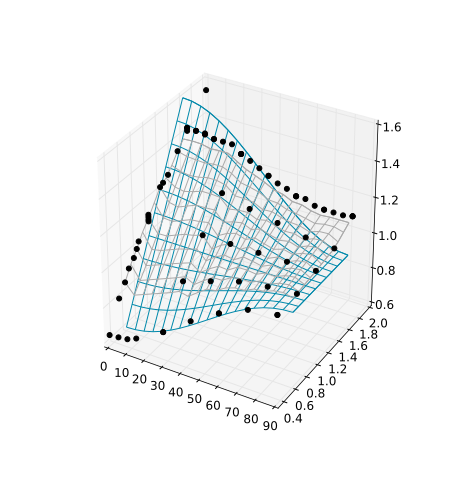
\includegraphics[width=\textwidth]{numvanal.png}
\caption{A comparison of the numerical results and the analytical theory shows
general agreement. Grey dots represent numerical simulation results, the grey surface represents an interpolating surface of the dots, and the blue surface represents the analytical model. Disagreement between the two may be due to edge effects and/or numerical
model convergence issues.}
\label{fig:numvanal}
\end{figure}

Additionally, preliminary measurements of both anisotropic salt/sugar
layered samples and of snow were taken. The anisotropic salt/sugar samples were
layered in roughly 1" thick layers at varying orientations relative to the
needle, while the snow measurements were taken with the needle at varying
orientations relative to the snowpack's horizontal plane.

Both models and measurements suggest that detecting anisotropy
in such materials is possible, though made difficult by variability between
measurements and the requirement of multiple measurements at various angles.
Further measurements will be required in order to develop a statistically sound
sample set, and further modeling will be required in order to establish a
sufficiently accurate model.

These studies do suggest that anisotropy in snow may be able to explain in part
the discrepancies between guarded hot plate and needle probe measurements in 
certain cases. In the case of alternating layers of snow, vertical conductivity
is always greater than horizontal conductivity due to the geometry of the
composite material, which would be expected to cause the opposite trend from
what is seen in the guarded hot plate/needle probe discrepancies.
\cite{lunardini} However, structural anisotropy, which may be caused by vapor
transport, could be sufficient explain the differences.

\bibliographystyle{agufull08}
\bibliography{report}
\end{document}
